%%%%%%%%%%%%%%%%%%%%%%%%%%%%%%%%%%%%%%%%%%%%%%%%%%%%%%%%%%%%%%%%%%%%%%%%%%%%%%%%
\section{Możliwości} %FIXME: mniej głupia nazwa
\subsection{Sprzęt}
\begin{frame}[fragile, allowframebreaks]{Coraz trudniej}
	\begin{block}{Zasada Moore'a}
		\begin{itemize}
			\item co kilkanaście miesięcy mamy do dyspozycji $2\times$ więcej tranzystorów.
			\item szkoda że od około 2003 nie ma co liczyć na przyspieszenie zegarów (,,frequency wall'').
			\item ,,memory wall'' - kiedyś dostęp do pamięci był tani, a obliczenia drogie. Teraz jest odwrotnie.
			\item ,,latency wall'': w czasie, kiedy wystarcza na podwojenie przepustowości procesorów/pamięci/dysków/sieci opóźnienia spadają tylko 1.2-1.3$\times$ (David A. Patterson : ,,Latency lags bandwith'')
			\item ,,speed wall'': $c \approx 3e8\frac{m}{s} \approx 10 \frac{cm}{clk}~@3GHz$ - w próźni
			\item na co wykorzystać tranzystory?
		\end{itemize}
	\end{block}
	\begin{block}{Decyzje}
		\begin{itemize}
			\item manycore vs. multicore
			\item RISC vs. CISC (wygodny pipeline vs. łatwo ręcznie; \verb*%x86%)
		\end{itemize}
	\end{block}
\end{frame}
%%%%%%%%%%%%%%%%%%%%%%%%%%%%%%%%%%%%%%%%%%%%%%%%%%%%%%%%%%%%%%%%%%%%%%%%%%%%%%%%
\begin{frame}[fragile]{Pamięć, cache}
	\begin{itemize}
		\item Prędkości (orientacyjnie):
		\begin{verbatim}
			reg ~       1clk
			L1  ~       3clk
			L2  ~      15clk
			L3  ~  50-100clk
			mem ~ 100-400clk
		\end{verbatim}
		\item Hierarchiczny cache (per-core, TLC: I\$ i D\$, współdzielony LLC, CC: MESI i pokrewne)
		\begin{itemize}
			\item HS vs. QS
			\item cachegrind
			\item cache oblivious algorithms
			\item \url{igoro.com/archive/gallery-of-processor-cache-effects/}
			\item page coloring
		\end{itemize}
		\item Hierarchiczny TLB
	\end{itemize}
\end{frame}
%%%%%%%%%%%%%%%%%%%%%%%%%%%%%%%%%%%%%%%%%%%%%%%%%%%%%%%%%%%%%%%%%%%%%%%%%%%%%%%%
\begin{frame}{Quicksort vs. Heapsort: wykorzystanie cache'a}
	\begin{figure}[h]
		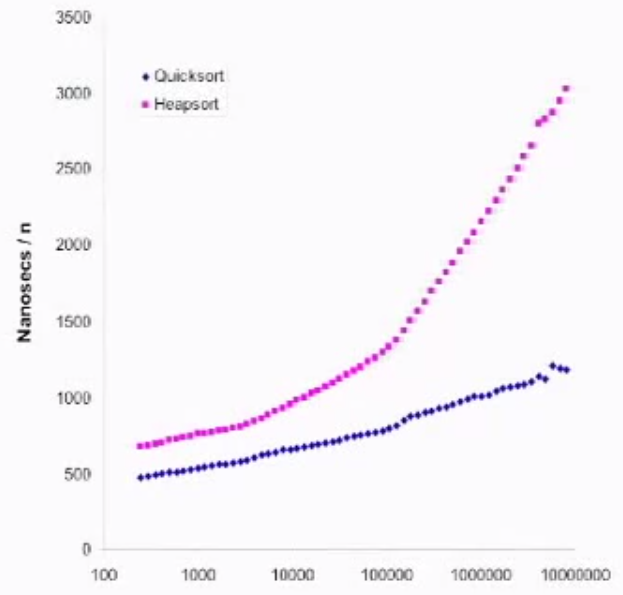
\includegraphics[width=0.6\textwidth]{gfx/cache_bentley}
		\caption{Źródło: Jon Bentley: ,,Three Beautiful Quicksorts'': \url{http://www.youtube.com/watch?v=QvgYAQzg1z8}}
	\end{figure}
\end{frame}
%%%%%%%%%%%%%%%%%%%%%%%%%%%%%%%%%%%%%%%%%%%%%%%%%%%%%%%%%%%%%%%%%%%%%%%%%%%%%%%%
\begin{frame}{Pipelining}
	\begin{figure}[h]
		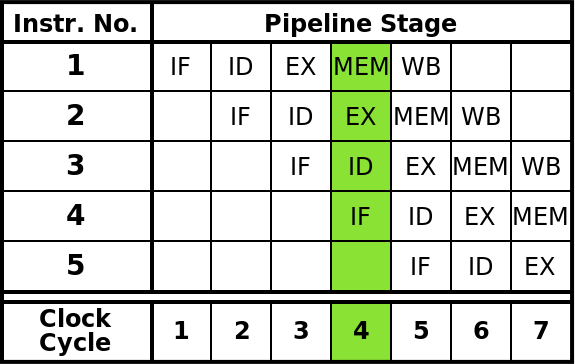
\includegraphics[width=0.6\textwidth]{gfx/pipelining}
		\caption{Źródło: \url{http://en.wikipedia.org/wiki/File:5_Stage_Pipeline.svg}}
	\end{figure}
\end{frame}
%%%%%%%%%%%%%%%%%%%%%%%%%%%%%%%%%%%%%%%%%%%%%%%%%%%%%%%%%%%%%%%%%%%%%%%%%%%%%%%%
\begin{frame}[fragile]{ILP}
	Static/dynamic ILP
	\begin{itemize}
		\item Pipelining (problem: branch == pipeline flush)
		\begin{itemize}
			\item inlining/unrolling
			\item delay slots
			\item branch predictor
			\item dependency detection (\verb*%a[i++]% vs. \verb*%a[++i]%)
			\item speculative execution, nadmiar rejestrow, store buffer/L0
			\item \verb*%CMOVcc%
			\item demo: himrbp
		\end{itemize}
		\item cache miss == pipeline stall: OOO, HW threads, superscalar
	\end{itemize}
	\tiny\url{http://www.infoq.com/presentations/click-crash-course-modern-hardware}
	\tiny\url{http://www.gamedev.net/page/resources/_/technical/general-programming/a-journey-through-the-cpu-pipeline-r3115}
\end{frame}
%%%%%%%%%%%%%%%%%%%%%%%%%%%%%%%%%%%%%%%%%%%%%%%%%%%%%%%%%%%%%%%%%%%%%%%%%%%%%%%%
\begin{frame}{SIMD}
	\begin{itemize}
		\item MMX - 64b
		\item SSE - 128b
		\item AVX - 256b
		\item MIC's VPU - 512b
	\end{itemize}
\end{frame}
%%%%%%%%%%%%%%%%%%%%%%%%%%%%%%%%%%%%%%%%%%%%%%%%%%%%%%%%%%%%%%%%%%%%%%%%%%%%%%%%
\begin{frame}[fragile]{x86\_64}
	\begin{block}{Nowości}
		\begin{itemize}
			\item Nowe rejestry: \textbf{SIMD} i \textbf{general purpose} (tych $2\times$ więcej niż w x86)
			\item Nowe instrukcje dla tychże
			\item Większe rejestry: większe zmienne, większa przestrzeń adresowa (tak wirtualna jak i fizyczna, tak w trybie 64-bitowym jak i w PAE)
			\item Śmielsze kompilatory
			\item Łatwiejsze tworzenie PIC: adresowanie wzgledem RIP
			\item Bit \texttt{NX}
		\end{itemize}
	\end{block}
\end{frame}
%%%%%%%%%%%%%%%%%%%%%%%%%%%%%%%%%%%%%%%%%%%%%%%%%%%%%%%%%%%%%%%%%%%%%%%%%%%%%%%%
\subsection{Język}
\begin{frame}[fragile, allowframebreaks]{,,Zachowania'' w C i pokrewnych językach}
	\begin{block}{Definicje}
		\small\begin{quote}
			The semantic descriptions in this International Standard define a \textbf{parameterized nondeterministic abstract machine}.

			Certain aspects and operations of the abstract machine are described in this International Standard as \textbf{implementation-defined} (for example, sizeof(int)). These constitute the parameters of the abstract machine. Each implementation shall include documentation describing its characteristics and behavior in these respects.

			Certain other aspects and operations of the abstract machine are described in this International Standard as  \textbf{unspecified} (for example, order of evaluation of arguments to a function). Where possible, this International Standard defines a set of allowable behaviors. These define the nondeterministic aspects of the abstract machine.

			Certain other operations are described in this International Standard as  \textbf{undefined} (for example, the effect of dereferencing the null pointer). [ Note: this International Standard imposes no requirements on the behavior of programs that contain undefined behavior. —end note ]
		\end{quote}
	\end{block}
	\begin{block}{W skrócie}
		\begin{figure}[h]
			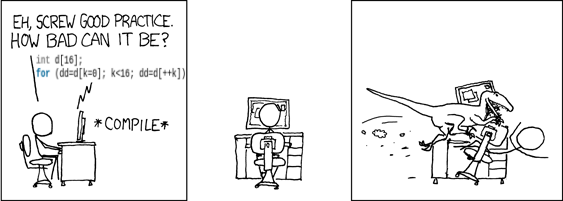
\includegraphics[width=0.8\textwidth]{gfx/undef_xkcd}
			\caption{Źródło: \url{http://xkcd.com/292/}, na licencji CC-BY-NC. kod: H.264 reference implementation.}
		\end{figure}
	\end{block}
	\begin{block}{IOCC, Underhanded C Contest}
		\begin{quote}
			If your source file is over 200 lines, you are not likely to win. You can hide a semi truck in 300 lines of C.
		\end{quote}
	\end{block}
\end{frame}
%%%%%%%%%%%%%%%%%%%%%%%%%%%%%%%%%%%%%%%%%%%%%%%%%%%%%%%%%%%%%%%%%%%%%%%%%%%%%%%%
\begin{frame}[fragile]{Konkretne przykłady tychże}
	\begin{block}{Punkty sekwencyjne, kolejność wykonania}
		\begin{itemize}
			\item czym są i co w nich jest ,,undefined''/,,unspecified''
			\item \lstinline[language=c]!foo() + bar() + baz();!,  \lstinline[language=c]!i = ++i;!
			\item vs. Java
			\item vs. \verb*%C++11%: zmiany (relacja ,,sequenced before'')
			\item dlaczego?
			\item dlaczego standard nie gwarantuje warningów?
		\end{itemize}
		\begin{figure}[h]
			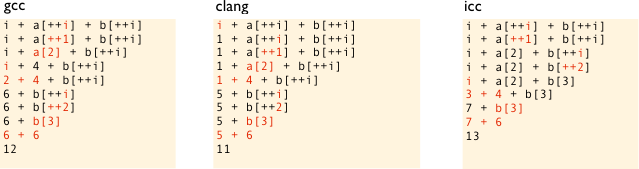
\includegraphics[width=0.75\textwidth]{gfx/unspec_compilers}
			\caption{ \tiny\url{http://www.pvv.org/~oma/UnspecifiedAndUndefined_ACCU_Apr2013.pdf}.}
		\end{figure}
	\end{block}
\end{frame}
%%%%%%%%%%%%%%%%%%%%%%%%%%%%%%%%%%%%%%%%%%%%%%%%%%%%%%%%%%%%%%%%%%%%%%%%%%%%%%%%
\begin{frame}[fragile, allowframebreaks]{Problemy z pamięcią}
	\begin{itemize}
		\item aliasing (vs. \texttt{FORTRAN}): wskaźniki vs. offsety, atrybuty, lokalność, \texttt{static}, \texttt{-fno-strict-aliasing}
		\item alignment
		\item Type Based Alias Analysis
		\item value representation (\verb*%true_true.c%)
		\item rationale
		\item \url{http://dbp-consulting.com/tutorials/StrictAliasing.html}
	\end{itemize}
\end{frame}
%%%%%%%%%%%%%%%%%%%%%%%%%%%%%%%%%%%%%%%%%%%%%%%%%%%%%%%%%%%%%%%%%%%%%%%%%%%%%%%%
\begin{frame}[fragile, allowframebreaks]{Jak C pomaga programiście pomóc sobie}
	\begin{itemize}
		\item \verb*%register%/\verb*%volatile%
		\item \verb*%static%
		\item \verb*%switch% - ,,most high-level feature of C''
		\item \verb*%restrict% (\verb*%C99%)
		\item \verb*%inline%/\verb*%const%/\verb*%constexpr%/\verb*%extern%
		\begin{itemize}
			\item vs. makra
			\item vs. \verb*%template% (unrolling)
			\item vs. rekursja, \verb*%&%, \verb*%vla%, \verb*%-fno-inline%
		\end{itemize}
		\item typy: jak (wg. standardu) ma się \verb*%int% do \verb*%long% i \verb*%short%? \verb*%<stdint.h>%, \verb*%int_fast*_t%
		\item RVO/copy elision
		\item \verb*%C++11%: \verb*%alignof%/\verb*%alignas%, \verb*%noexcept%, move semantics, optymalizacja exception handling
	\end{itemize}
\end{frame}
%%%%%%%%%%%%%%%%%%%%%%%%%%%%%%%%%%%%%%%%%%%%%%%%%%%%%%%%%%%%%%%%%%%%%%%%%%%%%%%%
\subsection{Biblioteki}
\begin{frame}[fragile]{Biblioteki}
	\begin{itemize}
		\item SSO
		\item COW (lazy copy)
		\item GPU
		\item nie zawsze należy ufać (,,Three Beautiful Quicksorts'')
		\item builtins
		\item problem z fuzją - Halide
	\end{itemize}
\end{frame}
%%%%%%%%%%%%%%%%%%%%%%%%%%%%%%%%%%%%%%%%%%%%%%%%%%%%%%%%%%%%%%%%%%%%%%%%%%%%%%%%
\subsection{Narzędzia}
\begin{frame}[fragile]{Narzędzia}
	\begin{itemize}
		\item profilery: \texttt{gprof}, \texttt{cachegrind}
		\item packery: \texttt{upx}
		\item kompilatory: \texttt{gcc-4.8}
		\begin{itemize}
			\item Generowany kod:
			\begin{itemize}
				\item \verb*%-p[g]%, PGO: \texttt{-fprofile-generate}, \texttt{-fprofile-use}
				\item \verb*%-g[gdb]% \verb*%-Og%, warningi
				\item \verb*%-O{0,1,2,3,s,fast}%, \verb*%-ffast-math%
				\item \verb*%-m{32,x32,64}%, \verb*%-mtune=*%, \verb*%-mfpmath={387,sse}%, \verb*%-m{96,128}bit-long-double%
				\item \url{http://gcc.gnu.org/onlinedocs/gcc-4.8.0/gcc/Optimize-Options.html}, \url{http://gcc.gnu.org/onlinedocs/gcc-4.8.0/gcc/i386-and-x86_002d64-Options.html}, \url{http://gcc.gnu.org/onlinedocs/gcc-4.8.0/gcc/Code-Gen-Options.html}
			\end{itemize}
			\item Informacje o generowanym kodzie
			\begin{itemize}
				\item \texttt{-fstack-usage}
				\item \texttt{-ftree-vectorizer-verbose=*}
				\item \texttt{-fdump-tree-\{vectorize,optimize\}=stderr=*}
				\item \texttt{-fopt-info-\{optimized,vec-missed\}=stderr=*}
			\end{itemize}
		\end{itemize}
	\end{itemize}
\end{frame}
%%%%%%%%%%%%%%%%%%%%%%%%%%%%%%%%%%%%%%%%%%%%%%%%%%%%%%%%%%%%%%%%%%%%%%%%%%%%%%%%
\begin{frame}[fragile, allowframebreaks]{Kompilator}
	\begin{block}{Intrinsics}
		Cień nadziei na szczątkową przenośność między procesorami, gorzej z kompilatorami.
		\begin{itemize}
			\item \verb*%__builtin_expect%
			\item \verb*%__builtin_cpu_supports("sse2")%
		\end{itemize}
		\url{http://gcc.gnu.org/onlinedocs/gcc-4.8.0/gcc/Vector-Extensions.html}
		\url{http://gcc.gnu.org/onlinedocs/gcc-4.8.0/gcc/X86-Built_002din-Functions.html}
	\end{block}
	\begin{block}{Language extensions}
		\begin{itemize}
			\item GCC: extended asm (ostrożnie, spill rejestrów)
			\item GCC: explicit reg vars
		\end{itemize}
	\end{block}
	\begin{block}{\texttt{\#pragma}}
		\begin{itemize}
			\item sztywna składnia
			\item OpenMP
			\item icc
		\end{itemize}
	\end{block}
\end{frame}
%%%%%%%%%%%%%%%%%%%%%%%%%%%%%%%%%%%%%%%%%%%%%%%%%%%%%%%%%%%%%%%%%%%%%%%%%%%%%%%%
\begin{frame}[fragile, allowframebreaks]{Kompilator}
	\begin{block}{Attributes}
		Wygodniejsza składnia, podobna konstrukcja w \texttt{C++11}
		\begin{itemize}
			\item \verb*%aligned%, \verb*%packed%
			\item \verb*%fastcall%
			\item \verb*%noreturn%
			\item \verb*%pure%, \verb*%malloc%
			\item \verb*%noinline%, \verb*%alwaysinline%
			\item \verb*%target% - multiversioning, demo w \texttt{vec.cpp}
			\item \url{http://gcc.gnu.org/onlinedocs/gcc-4.8.0/gcc/Function-Attributes.html}, \url{http://gcc.gnu.org/onlinedocs/gcc-4.8.0/gcc/Type-Attributes.html}, \url{http://gcc.gnu.org/onlinedocs/gcc-4.8.0/gcc/Variable-Attributes.html}
		\end{itemize}
	\end{block}
\end{frame}
